\documentclass[10pt,twocolumn,letterpaper]{article}

\usepackage{cvpr}
\usepackage{times}
\usepackage{epsfig}
\usepackage{graphicx}
\usepackage{amsmath}
\usepackage{amssymb}

% Include other packages here, before hyperref.

% If you comment hyperref and then uncomment it, you should delete
% egpaper.aux before re-running latex.  (Or just hit 'q' on the first latex
% run, let it finish, and you should be clear).
\usepackage[breaklinks=true,bookmarks=false]{hyperref}

\cvprfinalcopy % *** Uncomment this line for the final submission

\def\cvprPaperID{****} % *** Enter the CVPR Paper ID here
\def\httilde{\mbox{\tt\raisebox{-.5ex}{\symbol{126}}}}

% Pages are numbered in submission mode, and unnumbered in camera-ready
%\ifcvprfinal\pagestyle{empty}\fi
\setcounter{page}{1}
\begin{document}

%%%%%%%%% TITLE
\title{Machines are Among Us}

\author{Zach Minot\\
Georgia Institute of Technology\\
2nd Year Undergraduate, CS\\
{\tt\small zjminot@gatech.edu}
% For a paper whose authors are all at the same institution,
% omit the following lines up until the closing ``}''.
% Additional authors and addresses can be added with ``\and'',
% just like the second author.
% To save space, use either the email address or home page, not both
\and
Charles Gunn\\
Georgia Institute of Technology\\
2nd Year Undergraduate, CS \& Math\\
{\tt\small cgunn30@gatech.edu}
}

\maketitle
%\thispagestyle{empty}

%%%%%%%%% ABSTRACTcommunicate
\begin{abstract}
   The ABSTRACT is to be in fully-justified italicized text, at the top
   of the left-hand column, below the author and affiliation
   information. Use the word ``Abstract'' as the title, in 12-point
   Times, boldface type, centered relative to the column, initially
   capitalized. The abstract is to be in 10-point, single-spaced type.
   Leave two blank lines after the Abstract, then begin the main text.
   Look at previous CVPR abstracts to get a feel for style and length.
\end{abstract}

%%%%%%%%% BODY TEXT
\section{Introduction}
To what extent can neural network models communicate with each other and discover
each other's identity? How would they use this information in a competitive setting?
For example, in a social deduction game, players attempt to uncover each other's
hidden allegiance---typically with one "good" team and one "bad" team.
Players must utilize deductive reasoning to find the truth or instead
lie to keep their role hidden. In this paper, we explore 
if neural networks can be successfully trained to
compete in a scenario such as this, and how would the opposing parties interact
during the period of debate.
\subsection{Among Us}
Among Us is a currently popular social deduction game,
where the "imposters" attempt to sabotage and kill all of the "crewmates". Crewmmates have
to complete tasks and figure out who the imposters are and eliminate them before the imposters
win.
At certain points in the game, after periods of no direct communication, players 
debate the roles of each individual based on information previously acquired through
their personal experience. At the end of this discussion, every player votes on a single
player to be eliminated. The player with the most votes is eliminated, and if there
is a tie, no one is voted out. We chose to emulate this game based on
the overall simplicity of the two roles and the requirement of communication
for either party to succeed. If the crew do not exchange information 
and all vote the same person, 
the vote could result in a tie or a crew being eliminated.
If the imposters do not bluff, the crew can easily spot the liars among the group. 
This provides ample room to explore and experiment with the communication between
the two opposing parties.
\subsection{Adverserial Networks}
Within this design space, there are adversarial parties working against each other.
In the deep learning realm, adversarial situations appear in adversarial examples~\cite{AdverserialEx} and within GANs (generative adversarial networks)
~\cite{NIPS2014_5ca3e9b1}
In particular, the latter often designs a contest between two neural networks, in the form
of a zero-sum game.
We build upon these concepts and foundations in our work.
\subsection{Multi-agent Communication}
Inherently, a social deduction game requires multiple agents to be trained and contested.
This has been explored within the deep learning problem space with multi-agent subproblems.
Both cooperative~\cite{DBLP:journals/corr/FoersterAFW16}~\cite{DBLP:journals/corr/FoersterAFW16a} 
and adversarial ~\cite{DBLP:journals/corr/AbadiA16} communication has been experimented with,
showing that models can effective share and also selectively protect information.
We reference these approaches we generate active adversarial communication between 
neural network models.
\begin{figure*}
   \begin{center}
      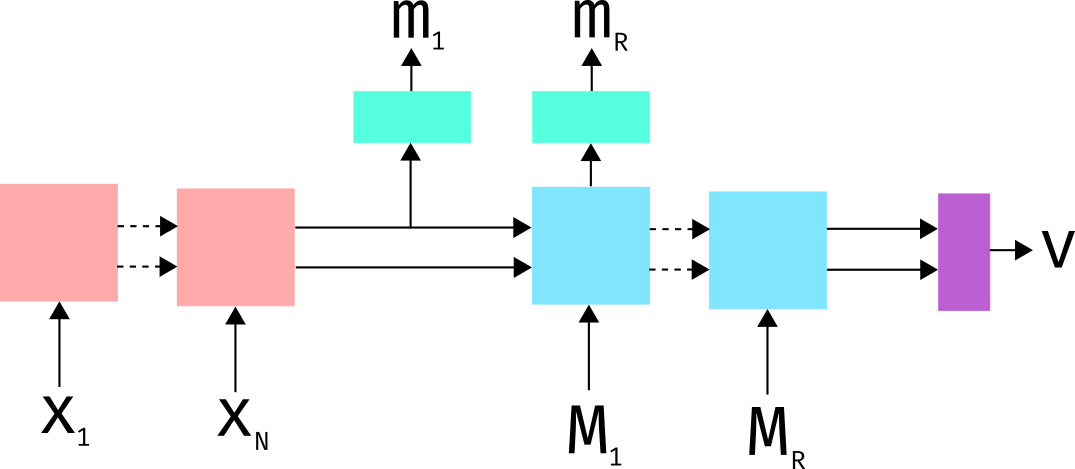
\includegraphics[width=0.8 \textwidth]{img/model.png}
   \end{center}
      \caption{Diagram of the Agent model. The red section is the perception LSTM,
      which takes in a sequence of events. The blue section is the communication
      LSTM, which recieves messages, and generates messages using the green MLP.
      Finally, the purple section is the voting MLP, which produces the agent's
      vote vector.}
   \label{fig:model}
\end{figure*}
\section{Approach}
In order to examine the interactions between multiple agents -- some of who are
secretly imposters who must ``lie'', we chose to construct an ``Among Us''-esque scenario
for our models to partake in. On a high level, we wanted each agent to 
first collect information
independant of the others. Then, there should be some phase of communication between the
models -- qualitatively, it is during this stage that the agents will attempt to
deduce who the imposters are, an the imposters will attempt to blend in. Finally, the
agents all vote on who they think is a likely imposter. The upcoming sections
explain how we chose to model each of these phases in greater detail.
\subsection{Deductive Situation}
During the period of communication in Among Us, the crew must do tasks
and gain information while the imposters must sabotage and kill the crew. We decided
to simplify the ``game'' by both removing the tasks and killing and making the entire
perception of each player predetermined. 

Specifically, each agent is given as input a matrix consisting
of $N$ events. During each event, the agent ``sees'' some subset of the other players
(sight is reflexive and symmetric, but not transitive).
They also may experience a ``sabotage'', which means they are in the prescence
of an imposter who is sabotaging. They cannot see the imposter, but the imposter
can see them during this event. Ultimately, each agent will recieve
a $N \times (P + 1)$ matrix, where $P$ is the total number of players -- the first
$P$ values of a row indicate who the agent is seeing, and the final value indicates
a sabotage.

These event matrices are generated randomly using four key parameters: the total number
of players ($P$), the number of those players who are imposters ($I$), the chance that
any given pair of players will see one another during an event (view chance), and the 
chance that any given imposter will sabotage during an  event (sabotage chance).

\subsection{Modeling Interpretation and Communication}
In order to process the input events, our agent model has an LSTM, which
generates $c_N$ and $h_N$, which are used as the initial inputs
$h_0$ and $c_0$ to the next phase:
communication. Communcation is also modeled with an LSTM. During each ``round''
of communication, every agent contributes a message vector of size $M$ via
a small MLP using $h_t$ as input. These messages are collected into a matrix
of size $M \times P$, which is fed as input into each agent's LSTM so that
their memory can be updated before the next round of communication -- there
are $R$ rounds in total. We chose
to model communication this way because it is a simple and symmetric way for the agents
to pass information between each other in multiple rounds.
   
\subsection{Zero-sum Target}
The last stage is the most simple one -- voting. The model simple takes the $h_R$ and
$c_R$ from the end of the communication LSTM and feeds them through
a small MLP finalized with a softmax layer. This results in a probability vector
of a confidence that a specific player should be ``voted out''.

At the end of voting, we calculate a ``crew score''. This score is simply the
maximum vote-off score that any imposter recieved, where votes
are averaged across all agents. Clearly, the imposters would like to minimize the
votes on themselves, so their loss function for training purposes is
simply the crew score. Inversely, the crew's loss function is the negation of
the crew score. This takes the form of a zero-sum game with similar application
as in generative adversarial networks.
\subsection{Training Scheme}
There were multiple decisions we had to make when attempting to train the models.
Imposter/Crew two different models, multitude of different hyperparameters and
sizes of inputs/outputs.
\subsection{Challenges}
The main challenge in building and running the model
came mainly in the form of training time, gradient overlap, 
and hyperparameter search. As discussed previously, to help speed up training time
and reduce gradient overlap between multiple different models training over the
same dataset, we had to only train either one imposter or crew, and keep the rest constant.
This limits the quick adaptivity, and may lead to the models attempting to train
against the constant tcooperative models ratrher than against the adversarial model.

Furthermore, the immense number of combinations of hyperparameters
and input and outputs sizes, along with no precedent for recommended values,
lead us to generalize our model significantly. Although this may seem like an ability for
customizability, it severely reduces reproducability over small changes. 

Another important challenge to recognize is the extreme "black box" architecture
of the model. With our current model iteration, we have no current approach to visualizing
exactly what the model is doing, especially with communication. Therefore there are
assumptions and estimations when creating conclusions about the model.
\subsection{Situation Hyperparameters}
To list the variable hyperparameters and input and outputs sizes for the player model,
overall, we have batch size, number of epochs, epoch length, the global LSTM hidden layer size, 
and the amount of players and imposters. For the perception phase, there is the
chance a player will view another player, the chance a sabotage occurs, and the number of $N$ events.  
The communication stage has variables the message size $M$ and the number of communication rounds
$R$.
\begin{figure*}
   \begin{center}
      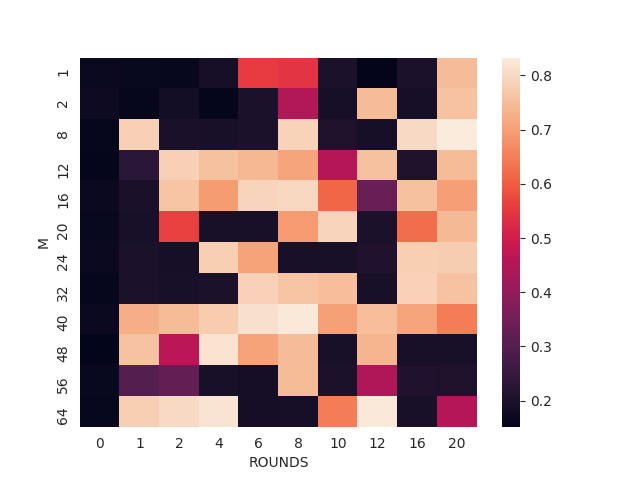
\includegraphics[width=0.8 \textwidth]{img/grid_search.png}
   \end{center}
      \caption{A grid search heat map over the size parameters M (message vector) 
      and Rounds (the number of communications) displaying the ending Crew score after 6 epochs.
      }
   \label{fig:model}
\end{figure*}
\section{Results}
% talk about our goal for a qualitatively "good" communication
% session.
\subsection{Oscillating Scores}
% talk about problems we saw frequently. show examples of "good" runs
% and bad runs

% grid search results.
\subsection{Model Evolution}
% are the agents "improving" or just changing minorly to trick each other
\subsection{Interpreting Communcation Vectors}
\subsection{Future Directions}
This approach is just a start into understanding how neural networks
communicate with one another. Although assumptions can be made,
understanding the actual information being transferred between each model is
a dark area. Innovative techniques must be found to analyze this information flow 
in order to fully comprehend the strategy within the game.

Furthermore, the results could help to explore more cryptographic use cases for neural networks.
It was observed that the crew could identify the imposters with no prior information which leads us to
believe the crew model had some sort of hidden code or tag to identify themselves.

Finally, similar work in adversarial networks could potentially give rise to
more techniques utilizing them. Generative adversarial networks are at the forefront of adversarial techniques, but possibly
large multi-agent adervasarial communication networks could give heed to more good results.
{\small
\bibliographystyle{ieee_fullname}
\bibliography{egbib}
}

\end{document}
